% Étude de la solution spécifique - H4413

\documentclass[twoside]{article}
\usepackage{hyperref}
\usepackage{eurosym}
\usepackage{slashbox}


\usepackage{graphicx}
\usepackage{subfig}
\usepackage{placeins}


% Unicode encoding  
\usepackage[utf8x]{inputenc}


% Colorfull Text
\usepackage{xcolor}


% \euro
\usepackage{eurosym}


% Language settings:
\usepackage[french]{babel}

\usepackage[T1]{fontenc}


% Tables
\usepackage{array}
\usepackage{longtable}


% Hyperrefferences  
\usepackage{hyperref}


\title{Étude de la solution spécifique}
\author{H4413}
% Page layout settings
\usepackage{geometry}
\geometry{
	a4paper,  % 21 x 29,7 cm
	body={160mm,240mm},
	left=30mm, 
	top=25mm,
	headheight=7mm, 
	headsep=4mm,
	marginparsep=4mm,
	marginparwidth=27mm
}


% Spacing:
\usepackage{setspace}


% Headers and footers:
\usepackage{fancyhdr}
\pagestyle{fancy}
          \fancyhf{}
          \fancyfoot[LE,RO]{\textcolor[gray]{0.3}{\thepage}}
          % Rulers width
          \renewcommand{\footrulewidth}{.3pt}
          \renewcommand{\headrulewidth}{.0pt}
\fancyfoot[LO,RE]{\textcolor[gray]{0.3}{H4413}}
\fancyfoot[CO,CE]{\textcolor[gray]{0.3}{Étude de la solution spécifique}}


% Vars & functs
% Paths
\newcommand\PIXPATH{./docs/pics}
\newcommand\SRCPATH{./docs/src}

% Object:
\newcommand\Object{Étude de la solution spécifique pour le remplacement du SI de la société GSTP}

% End of line(forced):
\newcommand\el{\hfill\\}

% Lists design:
\renewcommand{\labelitemi}{$\diamond$}
\renewcommand{\labelenumii}{\arabic{enumi}.\arabic{enumii}}


% Begining of the document
\begin{document}

	%Including all the files:

    % Fichier ./docs/tex/00.a.premiere_page.tex

% Front Page 

% Title:
\maketitle

\thispagestyle{empty}

\hfill\\
\vfill

% Picture

\begin{center}
    
\includegraphics[width=5cm]{\PIXPATH/frontPage}
\end{center}

\section*{Objet}
\Object

    % Fichier ./docs/tex/00.b.suivi.tex

% Suivi du document

% Modifications
\section*{Modifications du document}

\begin{center}
\begin{longtable}{|m{14mm}|m{36mm}|m{36mm}|m{60mm}|}
\hline
Version & Auteur & Date & Modification\endhead \hline
% Version
0
& % Auteur
& % Date
& % Modification
\\\hline
% Version
& % Auteur
& % Date
& % Modification
\\\hline
% Version
& % Auteur
& % Date
& % Modification
\\\hline
% Version
& % Auteur
& % Date
& % Modification
\\\hline
% Version
& % Auteur
& % Date
& % Modification
\\\hline
% Version
& % Auteur
& % Date
& % Modification
\\\hline
% Version
& % Auteur
& % Date
& % Modification
\\\hline
% Version
& % Auteur
& % Date
& % Modification
\\\hline
% Version
& % Auteur
& % Date
& % Modification
\\\hline

\end{longtable}
\end{center}

% Validations

\section*{Vérifications et validations du document}

\begin{center}
\begin{longtable}{|m{15mm}|m{36mm}|m{36mm}|m{60mm}|}
\hline
 & Responsable & Date & Remarques\endhead \hline
% Validé/vérifié par
& % Responsable
& % Date
& % Remarques
\\\hline
% Validé/vérifié par

& % Responsable

& % Date

& % Remarques

\\\hline
% Validé/vérifié par

& % Responsable

& % Date

& % Remarques

\\\hline
\end{longtable}
\end{center}

\pagebreak

    % Fichier ./docs/tex/00.c.toc.tex

% Table of contents 
\tableofcontents
\vfill
\pagebreak

    % Fichier ./docs/tex/1.Intro.tex


    % Fichier ./docs/tex/2.UseCases.tex

\section{Use cases}

On reproduit ici les cas d'utilisation de la solution spécifique modélisés
à l'aide d'ARIS.

\subsection{Achat}

\begin{center}
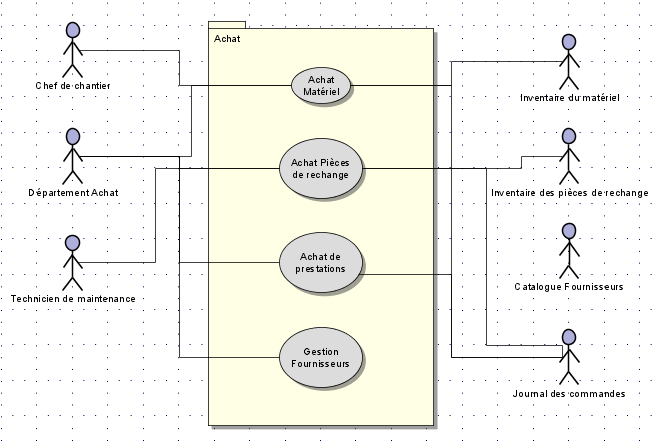
\includegraphics[width=10cm]{\PIXPATH/CasAchat}
\end{center}

\subsection{Maintenance}

\begin{center}
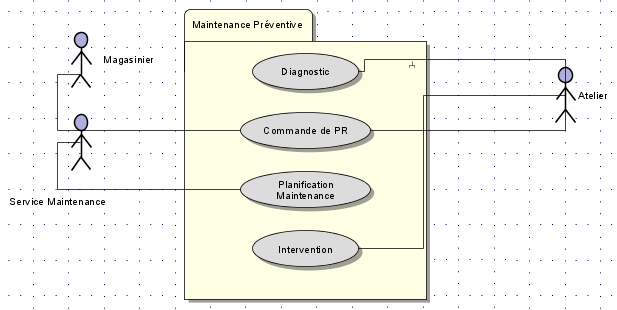
\includegraphics[width=10cm]{\PIXPATH/CasMaintenanceP}
\end{center}

\hfill\\

\begin{center}
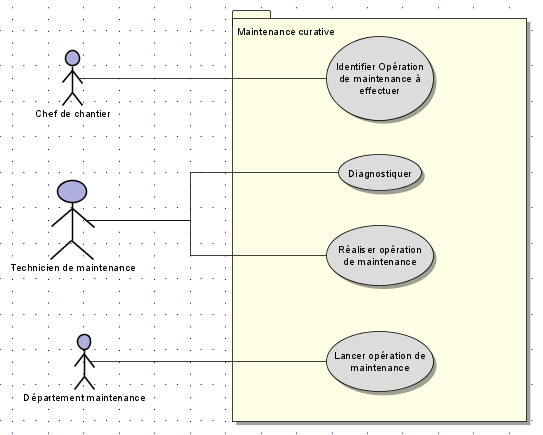
\includegraphics[width=10cm]{\PIXPATH/CasMaintenanceC}
\end{center}

\subsection{Utilisation}

\begin{center}
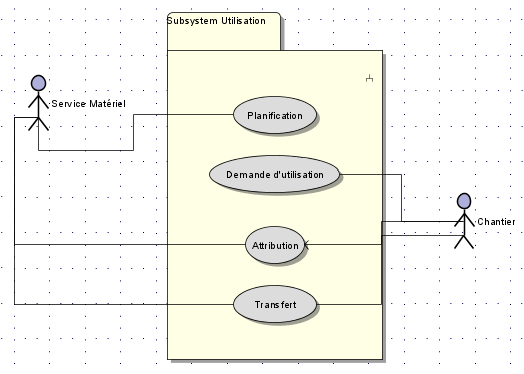
\includegraphics[width=10cm]{\PIXPATH/CasUtilisation}
\end{center}

    % Fichier ./docs/tex/3.FonctionsParAppli.tex

\section{Applications}

On présente ici la liste des fonctions de chaque application composant le
SI spécifique conçu pour GSTP.


\subsection{Fonctions globales}

L'ensemble des applications utilise une fonctionnalité de login, permettant
de restreindre l'accès à certains types d'utilisateurs.


\subsection{Application Achats}
% Communication avec la comptabilité pour les commandes
% Cette fonctionnalité est incluse dans les fonctions de commande, non ?

\begin{itemize}
\item Commander du matériel
\item Commander des pièces de rechange
\item Suivre une commande
\item Suivre le budget
\item Consulter le catalogue de fournisseurs (recherche de fournisseurs selon 
un ou plusieurs critères)
\item Editer le catalogue de fournisseurs :
	\begin{itemize}
	\item Création d'une fiche fournisseur
	\item Modification d'une fiche fournisseur
	\item Suppression d'une fiche fournisseur
	\end{itemize}
\end{itemize}

\subsection{Application Matériel}
\begin{itemize}
\item Récupération des plannings prévisionnels d'utilisation de matériels
des chantiers
\item Etablir le planning effectif d'affectation des
matériels pour les chantiers
\item Calculer et transmettre les factures qui correspondent à chaque chantier
à partir de l'utilisation des matériels
\item Enregistrer les mouvements de matériels (entrées et sorties du parc)
\item Évaluation de la valeur du parc
\end{itemize}


\subsection{Application Maintenance}
\subsubsection{Opérations de maintenance}
\begin{itemize}
\item Récupération de l'ensemble des demandes de maintenance exceptionnelle
des matériels
\item Etablir le planning pour la maintenance du matériel, prenant en
compte les maintenances préventives et curatives :
    \begin{itemize}
    \item planning global
    \item planning journalier
    \item anticipation de maintenances curatives
    \end{itemize}
\item Editer le catalogue et le  journal de maintenance pour chaque matériel :
    \begin{itemize}
    \item Consultation du catalogue de maintenance associé à une classe de 
    matériel
    \item Modification d'une fiche de maintenance associée à un matériel
     % A préciser
    \item Pas de création/suppression car la fiche de maintenance est liée
    au matériel auquel elle se réfère. La fiche de maintenance est donc
    créée puis supprimée automatiquement en même temps que le matériel dans
    la base.
    \end{itemize}
\end{itemize}

\subsubsection{Gestion du magasin de pièces de rechange}
\begin{itemize}
\item Fonctions de gestion d'un magasin :
    \begin{itemize}
    \item Suivre les entrées/sorties de pièces de rechanges
    \item Consultation du stock de pièces de rechange
    \end{itemize}
\item Traitement des commandes de pièces de rechange des chantiers :
    \begin{itemize}
    \item Enregistrement des commandes
    \item Optimisation de l'expédition hebdomadaire des commandes
    \item Suivi de la livraison 
    \end{itemize}
\item Commander des pièces de rechange auprès du Département Achat
\end{itemize}

\subsubsection{Gestion des techniciens de maintenance}
\begin{itemize}
\item Planification des affectations des techniciens de maintenance
\item Saisie des temps de travail des techniciens de maintenance
\end{itemize}


\subsection{Application Chantier}
L'application chantier reprend de nombreuses fonctionnalités de
l'application maintenance, adaptée et restreintes pour convenir à l'usage
d'un chantier.

\subsubsection{Fonctions transverses}
\begin{itemize}
\item Suivi du budget
\end{itemize}

\subsubsection{Matériel}
\begin{itemize}
\item Saisie du temps d'utilisation (hebdomaire)
\item Saisie de la prévision d'utilisation réelle du matériel (mensuelle)
\item Commander des pièces de rechange
\item Effectuer une demande de maintenance exceptionelle
\end{itemize}

\subsubsection{Personnel}
\begin{itemize}
\item Saisie du temps de travail des ouvriers
\item Planification des tâches assignées aux ouvriers
\end{itemize}

    % Fichier ./docs/tex/4.ListeObjetsMetier.tex

\section{Liste des objets métiers à développer}

La liste des objets métiers est présentée sous la forme d'un tableau à deux
entrées. De cette façon, on peut plus facilement voir quels sont les objets
métiers réutilisés plusieurs fois par différentes application.\\

\begin{center}
\begin{tabular}{|c|c|c|c|c|}
\hline
\backslashbox{Listes Objets Métiers}{Applications}&Achats& Matériel&Maintenance&Chantier\\
\hline
Affectation&&x&&x\\
\hline
Atelier&&x&x&\\
\hline
Chantier&&x&x&\\
\hline
Commande&x&x&x&x\\
\hline
Facture&&x&&x\\
\hline
Fonction&&&x&\\
\hline
Catalogue fournisseurs&x&&&\\
\hline
Fournisseur&x&&&\\
\hline
Gamme Maintenance&&&x&\\
\hline
Livraison&x&&&\\
\hline
Matériel&&x&x&x\\
\hline
Opération Maintenance&&&x&x\\
\hline
Période&&x&x&x\\
\hline
Piece Rechange&x&&x&x\\
\hline
Planification d'affectation&&x&x&x\\
\hline
Planification de maintenance&&x&x&\\
\hline
Poste Fonctionnel&x&x&x&x\\
\hline
Prestation&x&&&\\
\hline
Produit Acheté&x&&&\\
\hline
Regroupement de produits&&x&&\\
\hline
Type de matériel&&x&&\\
\hline
Type d'opération de maintenance&&&x&\\
\hline
Type de période&x&x&x&x\\
\hline
Type de prestation&x&&&\\
\hline
Type de regroupement de produit&&x&&\\
\hline
\end{tabular}
\end{center}

\end{document}

    % Fichier ./docs/tex/5.Techniques.tex

\section{Architecture Technique}
L'amélioration du système d’information de l'entreprise passe tout d'abord
par une augmentation du nombre de postes informatiques. Toutes les
informations passeront par le système informatique et seront enregistrées.

\subsection{Schéma}

\begin{figure}[!h]
\begin{center}
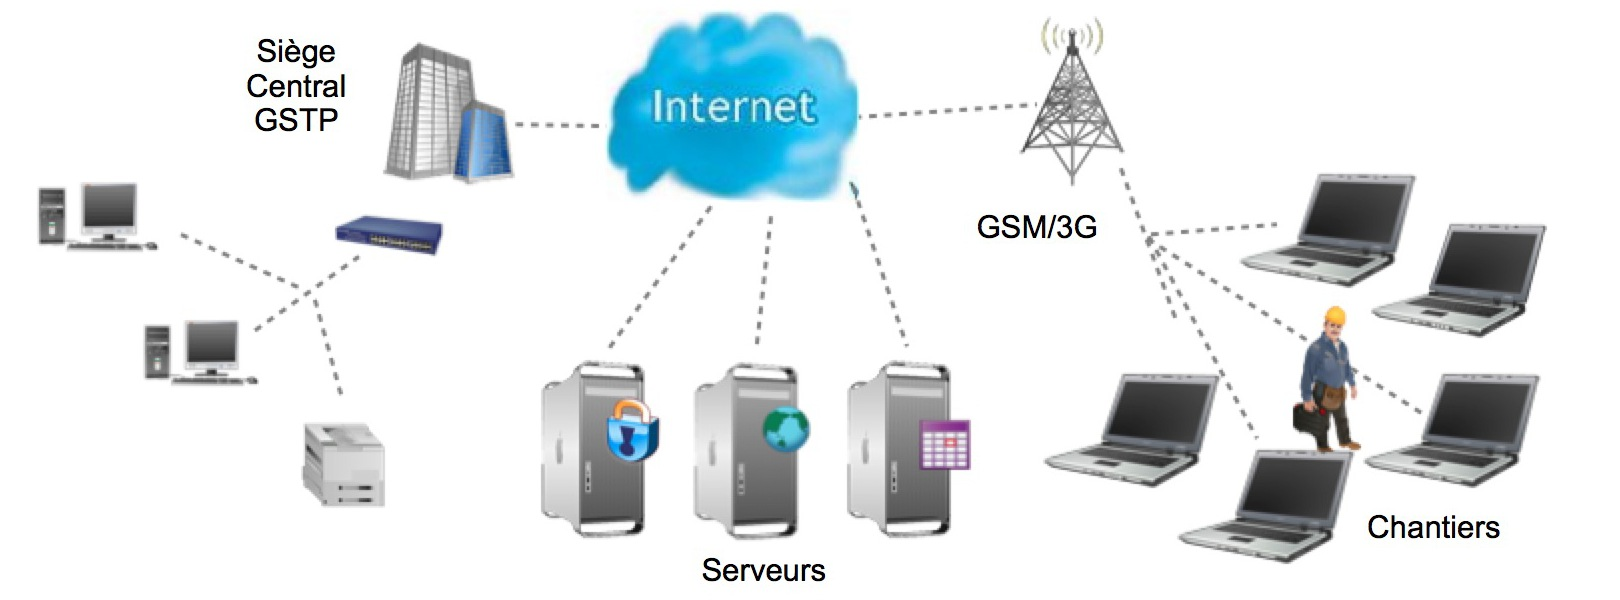
\includegraphics[width=13cm]{\PIXPATH/architech}
\caption{Schéma de l'organisation globale du SI}
\end{center}
\end{figure}


\subsection{Serveur}

Le serveur sera externalisé et il servira de support pour la base de
données et la gestion des accès à ces données. 

Chaque application, et donc chaque poste, sera configurée pour se connecter
à la base de données du serveur.  Toutes partageront les mêmes informations
et il sera ainsi possible de facilement faire le rapprochement entre les
achats et le matériel réceptionné par exemple.

	\subsubsection{Architecture}
Nous avons besoin d'un serveur d'application qui hébergera les applications
pour le chantier, le magasin, et les différents départements,  ainsi qu'une
base de données pour les information concernant aux chantiers, magasin,
fournisseurs, etc. 

Pour établir la communication client-serveur on utilisera le protocole
LDAP. Il fournit à l'utilisateur des commandes pour se connecter ou se
déconnecter,  pour rechercher, comparer, créer, modifier ou effacer des
entrées.  Des mécanismes de chiffrement (SSL ou TLS) et d'authentification
(SASL), couplés à des mécanismes de règles d'accès (ACL) permettent de
protéger les transactions et l'accès aux données.

	\subsubsection{Hébergement}
    Il nous faut un ensemble de serveurs capables de répondre à un grand
    nombre de requêtes, et ce en permanence.

Une solution consiste à héberger nos serveurs dans le \textsl{cloud}, on
utilisera le modèle IAAS pour  que l'entreprise maintient ses applications,
les {\sl runtimes}, l'intégration SOA, les bases de données, le logiciel
serveur.  Cette solution nous permettant ainsi de payer uniquement les
ressources que nous consommons, tout en bénéficiant d'une bonne résilience
aux pannes et d'une bonne disponibilité.  L'entreprise GoGrid fournit un
tel service, à partir de 60 \euro par mois.


\subsection{Communication}
Le département Achat, Matériel et Maintenance doivent être en réseau locale
pour qu'ils puissent  communiquer entre elles.

Sur les chantiers, il faut pouvoir relier les ordinateurs au siège par
l'intermédiaire d'Internet.  Nous savons que les chantiers sont souvent
amenés à se déplacer dans le cadre de leur travail, donc le réseau 3G est
indispensable pour qu'ils puissent être plus réactif vis-à-vis de leur
activité, comme par exemple, répondre instantanément à un email, rechercher
une information, ou échanger et communiquer sur une messagerie. 

Chaque poste disposera d’une clé 3G pour se connecter au réseau GSM haut
débit.

Il existe une large choix de formules proposées par les différents
opérateurs de téléphones portables, pour citer quelques unes :

Forfait journée : connexion n'importe quand durant tout la journée. Prix: 2 à
12 \euro

Forfait mois illimités : navigation par nombre d'heures illimitées.  Prix:
de 30 \euro à 70 \euro


\subsection{Chantiers}
On ajoutera 30 PC avec des caractéristiques qui correspondent au milieu de
travail (des ordinateurs résistantes au pression, vibration, humidité, etc.
1 pour chaque chantier), ces ordinateurs n'ont pas besoin d’être très
puissants, seulement ils doivent se connecter à internet et être capable de
faire fonctionner l'application de chantier.

Exemple : DELL ATG D620: PC Portable qui résiste l'humidité, l'altitude,
pression, et vibration, protégé contre les coups.
	
	Caractéristiques:

	\begin{enumerate} \item 14,1 puces \item lumineux \item sans reflet
	\item RAM 4 Go, Core 2 Duo T7600 \item 80 Go, 4200 T/M Anti-choc
	\item Windows Vista \item 2,8 Kg \end{enumerate}

Prix : 499 \euro 

    % Fichier ./docs/tex/6.CCL.tex


% The end
\end{document}

